\documentclass{article}
\usepackage{amsmath}
\usepackage{amssymb}
\usepackage{graphicx}
\usepackage{hyperref}
\usepackage[version=4]{mhchem}


\begin{document}
\section*{Problem}
Given \(\triangle A B C, \angle A=90^{\circ} . A B=A C . M\) is the midpoint of \(A C . A E \perp\) \(B M\) with the feet at \(E\). Extend \(A E\) to meet \(B C\) at \(D\). Prove that \(\angle A M B=\angle C M D\).\\
\centering
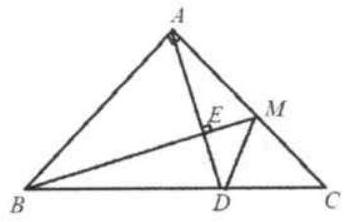
\includegraphics[width=\textwidth]{images/066(2).jpg}

\section*{Solution}
Draw the angle bisector of \(\angle A\) to meet \(B M\) at \(G\) and \(B C\) at \(H\).\\
Since \(A B=A C, \angle A=90^{\circ}, \angle B A G=45^{\circ}\).\\
\(\angle E B A=90^{\circ}-\angle E A B=90^{\circ}-(\angle B A G+\angle E A G)=90^{\circ}-\) \(\left(45^{\circ}+\angle E A G\right)=45^{\circ}-\angle E A G=\angle C A D\).

In \(\triangle A B G\) and \(\triangle A D C\), since \(\angle E B A=\angle C A D, \angle B A G=\angle C\),\\
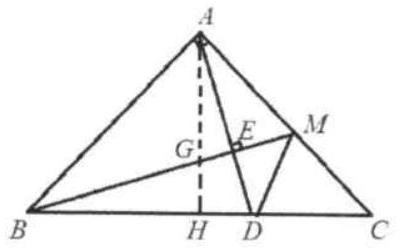
\includegraphics[width=\textwidth]{images/071.jpg} \(A B=A C, \triangle A B G \cong \triangle A D C\). Thus \(A G=C D\).\\
In \(\triangle A M G\) and \(\triangle C M D\), since \(\angle G A M=\angle D C M=45^{\circ}, A M=C M, A G=C D\), \(\triangle A M G \cong \triangle C M D\). Thus \(\angle A M B=\angle C M D\).

\end{document}
